\problemname{Lane Switching}

The Autonomous Car Manufacturer (ACM) needs to design algorithms to
control their cars.  One particular problem is lane switching---if the
car needs to switch lanes, it wants to do so in the safest manner.

Initially the car is in the leftmost lane, and the car needs to switch
to the rightmost lane.  The car has a variety of sensors and can
obtain the locations of all cars in a section of the highway.  When
the car needs to switch lanes, it takes a snapshot of the sensor
readings and design a plan to switch lanes based on the snapshot.  The
sensors have limited range.  All sensor readings will be distances
from the start of the sensor range.  For safety reason, the areas
outside of the sensor range are assumed to be occupied by cars.

% Each car has a length, and its location is given by the lane number
% (starting at 0 from the leftmost lane) and the distance of the car
% from the beginning of the lane.  

You may assume that all other cars are travelling at exactly the speed
limit.  However, the ACM would like to set itself apart by producing
cars that may drive at any speed regardless of the speed limit, as
long as it does not hit any other car.  For safety reasons, a lane
switch is always done while driving at the speed limit.

When a lane switch occurs, the destination must have unoccupied space
for the car to move into (a perfect fit is allowed).  
We define the safety factor of the plan as the closest distance to any
car while executing the plan.
% We define the
% safety factor of a lane switch as the closest distance to any car
% during the lane switch.  
We are only concerned about cars in the same lane, and will ignore
distances between cars in different lanes.  Obviously, the ACM
wants its cars to choose a plan that has the highest safety factor.

The first sample input is illustrated below.
\begin{center}
    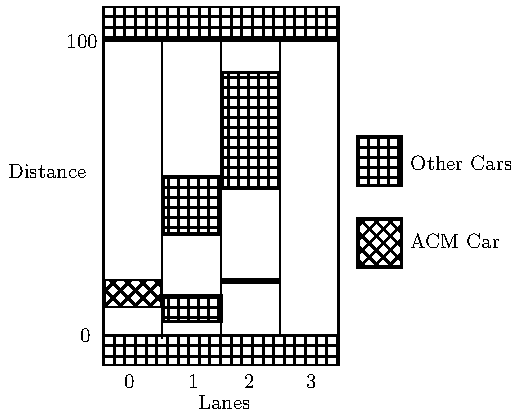
\includegraphics[width=0.75\textwidth]{figure.pdf}
\end{center}
\section*{Input}

The first line of input contains three integers $N$
($2 \leq N \leq 100$), $M$ ($M \geq 1$), $R$
($1 \leq R \leq 1\,000\,000$) indicating the number of lanes, the
number of cars on the road, and the sensor range.  The next $M$ lines
describe each car with three integers: the lane number (between 0 and
$N-1$, inclusive), the length of the car (positive), and the
distance from the start of the sensor range to the back of the car.
The distance is non-negative and at most $R$.  The first car given is
the ACM car.  Lane 0 is the leftmost lane, and lane $N-1$ is the
rightmost lane.

There are at most 100 cars in each lane.  No two cars will overlap
although they may touch bumper-to-bumper.


\section*{Output}

If the ACM car can switch from lane 0 to lane $N-1$, print a single
number indicating the maximum achievable safety factor.  Otherwise,
print \texttt{Impossible}.  Your answer will be considered correct if
its absolute error does not exceed $10^{-5}$.
